%%%%%%%%%%%%%%%%%%%%%%%%%%%%%%%%%%%%%%%%%%%%%%%%%%%%%%%%%%%%%%%%%%
%Packages
\documentclass[12pt, a4]{article}
\usepackage[top=3cm, bottom=4cm, left=3.5cm, right=3.5cm]{geometry}
\usepackage{tabularx}
\usepackage[utf8]{vietnam}
\usepackage[vietnamese]{babel}
\usepackage{float}
\usepackage{lastpage}
\usepackage[dvipsnames]{xcolor}
\usepackage{longtable,booktabs,array}
\usepackage{amsmath,amssymb}
\usepackage{lmodern}
\usepackage[T1]{fontenc}
\usepackage{setspace}
\usepackage{hyperref}
\usepackage{multirow}
\usepackage[framemethod=TikZ]{mdframed}
\usepackage{enumerate}
\usepackage[shortlabels]{enumitem}
\usepackage{fancyhdr}
\usepackage{indentfirst}
\usepackage{listings}
\usepackage{sectsty}
\usepackage{makecell}
\usepackage{booktabs}
\usepackage{hyperref}
\usepackage{titlesec}
\usepackage{color}
\usepackage{diagbox} 

\titlelabel{\thetitle.\quad}

\hypersetup{
    colorlinks=true,
    linkcolor=blue,
    filecolor=magenta,      
    urlcolor=blue,
}

\graphicspath{ {figures/} }



%%%%%%%%%%%%%%%%%%%%%%%%%%%%%%%%%%%%%%%%%%%%%%%%%%%%%%%%%%%%%%%%%%
%%%%%%%%%%%%%%%%%%%%%%%%%%%%%%%%%%%%%%%%%%%%%%%%%%%%%%%%%%%%%%%%%%

%Page setup
\pagestyle{fancy}
\headheight 35pt
\lhead{DS317.P11} % <-- class name
\rhead{
\includegraphics[width=0.9cm]{figures/UIT_Logo.png}} % <-- school logo(please upload the file first, then change the name here)
\lfoot{}
\pagenumbering{arabic}
\cfoot{\small\thepage}
\rfoot{}
\headsep 1.2em

\renewcommand{\baselinestretch}{1.25}       
\mdfdefinestyle{theoremstyle}{%
linecolor=black,linewidth=1pt,%
frametitlerule=true,%
frametitlebackgroundcolor=gray!20,
innertopmargin=\topskip,
}

%Code block setup
\definecolor{dkgreen}{rgb}{0,0.6,0}
\definecolor{gray}{rgb}{0.5,0.5,0.5}
\definecolor{mauve}{rgb}{0.58,0,0.82}

\lstset{frame=tb,
  language=python,
  aboveskip=3mm,
  belowskip=3mm,
  showstringspaces=false,
  columns=flexible,
  basicstyle={\small\ttfamily},
  numbers=none,
  numberstyle=\tiny\color{gray},
  keywordstyle=\color{blue},
  commentstyle=\color{dkgreen},
  stringstyle=\color{mauve},
  breaklines=true,
  breakatwhitespace=true,
  tabsize=3
}

% Redefine \texttt to use blue color
\let\oldtexttt\texttt
\renewcommand{\texttt}[1]{\textcolor{blue}{\oldtexttt{#1}}}
%%%%%%%%%%%%%%%%%%%%%%%%%%%%%%%%%%%%%%%%%%%%%%%%%%%%%%%%%%%%%%%%%%
%%%%%%%%%%%%%%%%%%%%%%%%%%%%%%%%%%%%%%%%%%%%%%%%%%%%%%%%%%%%%%%%%%
%Begin now!



\begin{document}
\begin{titlepage}
    \begin{center}
        \begin{centering}
            \textsc{\LARGE Đại học quốc gia TP.HCM}
        
            
% \newline
\textsc{\LARGE Trường đại học công nghệ thông tin}\\[1cm] 
        
        
\includegraphics[scale=0.25]{figures/UIT_Logo.png}\\[1.0cm]
        

% Môn học
\textsc{\large \textbf{Môn học}: Khai phá dữ liệu trong doanh nghiệp}\\[0.5cm] 
\textsc{\large Lớp: DS317.P11}\\[1cm] 

%----------------------------------------------------------------------------------------
%	TITLE
%----------------------------------------------------------------------------------------

% \hrule \\[0.4cm]
{\huge \bfseries Báo cáo đề tài}\\[0.3cm]
{\large \textbf{GVHD}: ThS. Nguyễn Thị Anh Thư}\\[1cm] 

 
%----------------------------------------------------------------------------------------
%	TÁC GIẢ 
%----------------------------------------------------------------------------------------
\emph{\centering Nhóm sinh viên thực hiện:}\\[0.5cm]
\begin{minipage}{0.35\textwidth}
\begin{flushleft} \large
Nguyễn Hữu Nam		\\
Nguyễn Khánh 			\\
Võ Đình Khánh			\\
Nguyễn Minh Sơn		\\
Bùi Hồng Sơn			\\
\end{flushleft}
\end{minipage}
~
\begin{minipage}{0.3\textwidth}
\begin{flushright} \large
    MSSV: 22520917 \\
    MSSV: 22520641\\
    MSSV: 22520659\\
    MSSV: 22521254\\
    MSSV: 22521246\\
\end{flushright}
\end{minipage}
    \end{centering}
    \end{center}
\end{titlepage}

% ----------------------------------------------------------------------------------------
\newpage
\tableofcontents
\newpage
% 1.----------------------------------------------------------------------------------------

\section{Tổng quan}

Khai phá dữ liệu, đặc biệt là dữ liệu lớn, đã trở thành một lĩnh vực nghiên cứu quan trọng và thu hút sự quan tâm của các nhà khoa học trong những năm gần đây. Các ứng dụng của khai phá dữ liệu rất đa dạng, được triển khai trong nhiều lĩnh vực như kinh doanh, giáo dục, y tế, tài chính, và ngân hàng. Đặc biệt, khai phá dữ liệu trong giáo dục, cụ thể là khai phá dữ liệu lớn, đang là chủ đề thu hút nhiều nghiên cứu nhờ vào tính ứng dụng cao và tiềm năng cải thiện chất lượng giáo dục.

Trong bối cảnh giáo dục trực tuyến hiện nay, người học cần phải tự chủ động và có tinh thần tự giác cao do số lượng môn học đa dạng thuộc nhiều lĩnh vực khác nhau. Họ cần phân bổ thời gian học tập hợp lý cho từng nhóm môn học nhằm bổ sung và nâng cao kiến thức chuyên ngành cần thiết. Tuy nhiên, các nền tảng học tập trực tuyến thường không có ràng buộc cụ thể về thời gian và điểm số, dẫn đến tình trạng nhiều khóa học không được hoàn thành đúng thời hạn, thậm chí bị bỏ dở do người học mất hứng thú.

Vì vậy, công tác cố vấn học tập trên các nền tảng trực tuyến trở nên vô cùng quan trọng để giúp người học cải thiện hiệu suất học tập và gợi ý các khóa học phù hợp với nhu cầu cá nhân. Đây là một bài toán thuộc lĩnh vực khai phá dữ liệu, đặc biệt khi xử lý với số lượng lớn dữ liệu liên quan đến người học và hành vi học tập của họ. Việc nghiên cứu và xây dựng hệ thống khuyến nghị khóa học góp phần quan trọng vào việc cá nhân hóa trải nghiệm học tập, hỗ trợ người dùng lựa chọn các khóa học phù hợp với mục tiêu và nhu cầu học tập.

\subsection{Định nghĩa và ngữ cảnh bài toán}

Trong bối cảnh các nền tảng học tập trực tuyến, người học thường gặp khó khăn trong việc lựa chọn khóa học phù hợp. Điều này đặt ra nhu cầu xây dựng một hệ thống khuyến nghị giúp cá nhân hóa quá trình học tập của từng người. Bài toán được định nghĩa với đầu vào và đầu ra như sau:

\begin{itemize}
    \item \textbf{Input}: Dữ liệu lớn từ các nền tảng học tập trực tuyến, bao gồm thông tin về người học, thông tin khóa học, và dữ liệu về các hoạt động học tập của người dùng.
    \item \textbf{Output}: Đề xuất top-$k$ khóa học phù hợp nhất với người dùng (trong đó $k \in \mathbb{N}^*$, ví dụ trong nghiên cứu này $k=10$).
\end{itemize}

\subsection{Ứng dụng}

Bài toán khuyến nghị khóa học cho các nền tảng học tập trực tuyến có nhiều ứng dụng thực tiễn, bao gồm:
\begin{itemize}
    \item \textbf{Cá nhân hóa quá trình học tập}: Hệ thống giúp người học lựa chọn các khóa học phù hợp với nhu cầu và trình độ, từ đó cá nhân hóa lộ trình học tập.
    \item \textbf{Tăng tỷ lệ hoàn thành khóa học}: Đề xuất khóa học phù hợp giúp người học duy trì động lực học tập, từ đó tăng tỷ lệ hoàn thành khóa học.
    \item \textbf{Tối ưu hóa lộ trình học tập}: Gợi ý các khóa học tiếp theo dựa trên kỹ năng hiện tại và các khóa học đã hoàn thành.
    \item \textbf{Ứng dụng trong đào tạo doanh nghiệp}: Hỗ trợ doanh nghiệp xây dựng chương trình đào tạo nhân viên hiệu quả, phù hợp với mục tiêu phát triển nghề nghiệp.
    \item \textbf{Nâng cao hiệu quả sử dụng tài nguyên}: Giúp người học tiết kiệm thời gian và tập trung vào các khóa học có giá trị cao.
\end{itemize}

\subsection{Khó khăn và thách thức}

Mặc dù có nhiều tiềm năng, bài toán khuyến nghị khóa học vẫn gặp phải các khó khăn và thách thức như:
\begin{itemize}
    \item \textbf{Chất lượng và sự đa dạng của dữ liệu}: Dữ liệu không đồng nhất hoặc không đầy đủ, gây khó khăn trong phân tích hành vi người học.
    \item \textbf{Xử lý dữ liệu lớn}: Khối lượng dữ liệu lớn đòi hỏi khả năng tính toán mạnh mẽ và các thuật toán tối ưu.
    \item \textbf{Lựa chọn đặc trưng quan trọng}: Việc chọn lọc các đặc trưng phù hợp từ bộ dữ liệu lớn đòi hỏi sự cân nhắc về tài nguyên và thời gian.
    \item \textbf{Đánh giá mô hình}: Thiếu dữ liệu rõ ràng về mức độ hài lòng của người học, khiến việc đánh giá hệ thống trở nên khó khăn.
\end{itemize}

\subsection{Các nghiên cứu liên quan}

Các phương pháp khuyến nghị chính bao gồm:
\begin{itemize}
    \item \textbf{Matrix Factorization}: Phân rã ma trận để tìm các yếu tố tiềm ẩn.
    \item \textbf{Collaborative Filtering}: Sử dụng thông tin tương đồng giữa người dùng hoặc khóa học.
    \item \textbf{Content-Based Filtering}: Gợi ý dựa trên nội dung và đặc trưng của khóa học.
    \item \textbf{Hybrid Systems}: Kết hợp nhiều phương pháp để tăng hiệu quả.
    \item \textbf{Graph-Based Methods}: Sử dụng đồ thị để biểu diễn mối quan hệ giữa người dùng và khóa học.
    \item \textbf{Neural Collaborative Filtering}: Ứng dụng Deep Learning để học các tương tác phi tuyến.
\end{itemize}

\section{Các công trình nghiên cứu liên quan}

Trong lĩnh vực khuyến nghị khóa học, nhiều công trình nghiên cứu đã được thực hiện nhằm cải thiện hiệu quả và độ chính xác của các hệ thống khuyến nghị. Một số phương pháp nổi bật được đề xuất như sau:

\subsection{Matrix Factorization}

Matrix Factorization (MF) là một kỹ thuật phổ biến trong hệ thống khuyến nghị, được sử dụng để phân rã ma trận user-item nhằm phát hiện các yếu tố tiềm ẩn ảnh hưởng đến hành vi của người dùng. Koren và cộng sự (2009) đã giới thiệu phương pháp này và áp dụng vào hệ thống khuyến nghị, đặc biệt trong bài toán đề xuất phim. Phương pháp này cho phép mô hình hóa sự tương tác giữa người dùng và các khóa học dựa trên các đặc trưng tiềm ẩn, mang lại kết quả tốt trong nhiều bài toán thực tế.

\subsection{Collaborative Filtering}

Collaborative Filtering (CF) là một trong những phương pháp lâu đời nhất và hiệu quả nhất trong khuyến nghị. CF được chia thành hai nhánh chính:
\begin{itemize}
    \item \textbf{User-User Collaborative Filtering}: Dựa trên sự tương đồng giữa các người dùng để gợi ý các khóa học mà người dùng có thể quan tâm.
    \item \textbf{Item-Item Collaborative Filtering}: Dựa trên sự tương đồng giữa các khóa học để gợi ý các khóa học mới cho người dùng.
\end{itemize}
Su và Khoshgoftaar (2009) đã thực hiện một khảo sát toàn diện về CF và các phương pháp cải tiến nhằm khắc phục những hạn chế của nó, bao gồm vấn đề thưa thớt dữ liệu và mở rộng quy mô.

\subsection{Content-Based Filtering}

Content-Based Filtering (CBF) là phương pháp tập trung vào các đặc trưng của khóa học, dựa trên thông tin về nội dung của các khóa học mà người dùng đã tham gia để đưa ra gợi ý. Burke (2002) đã tổng hợp các phương pháp CBF và chỉ ra rằng việc kết hợp các đặc trưng nội dung của khóa học và hành vi người dùng có thể nâng cao hiệu quả gợi ý.

\subsection{Hybrid Recommender Systems}

Hybrid Recommender Systems là sự kết hợp giữa Collaborative Filtering và Content-Based Filtering nhằm khắc phục những hạn chế của từng phương pháp riêng lẻ. Burke (2002) đã thực hiện một nghiên cứu toàn diện về các hệ thống khuyến nghị lai, cho thấy rằng việc tích hợp các phương pháp có thể cải thiện hiệu quả và tính tổng quát của hệ thống.

\subsection{Graph-Based Recommender Systems}

Phương pháp dựa trên đồ thị (Graph-Based Recommender Systems) sử dụng cấu trúc đồ thị để biểu diễn mối quan hệ giữa người dùng và khóa học. Các thuật toán như Random Walk hoặc PageRank được áp dụng để tìm kiếm và khai thác các kết nối trong dữ liệu. Phương pháp này đặc biệt hiệu quả khi xử lý dữ liệu phức tạp với nhiều mối quan hệ đa chiều.

\subsection{Neural Collaborative Filtering}

Neural Collaborative Filtering (NCF) là một hướng tiếp cận hiện đại, kết hợp Collaborative Filtering với Deep Learning để học các tương tác phi tuyến giữa người dùng và khóa học. He và cộng sự (2017) đã giới thiệu mô hình NCF và cho thấy hiệu suất vượt trội của nó so với các phương pháp truyền thống trong các tập dữ liệu lớn và phức tạp.

\subsection{Các hệ thống khuyến nghị khóa học dựa trên dữ liệu lớn}

Trong bối cảnh dữ liệu lớn, các nền tảng như MOOCCubeX cung cấp một lượng dữ liệu khổng lồ về hành vi học tập của người dùng. Zhang và cộng sự (2022) đã phát triển một hệ thống khuyến nghị dựa trên dữ liệu từ MOOCCubeX, sử dụng các mô hình đồ thị để cá nhân hóa lộ trình học tập. Kết quả cho thấy hệ thống có khả năng gợi ý các khóa học phù hợp và tăng tỷ lệ hoàn thành khóa học.

\subsection{Ứng dụng của các mô hình học sâu}

Học sâu (Deep Learning) được áp dụng rộng rãi trong các hệ thống khuyến nghị khóa học hiện đại. Các mạng nơ-ron tích chập (Convolutional Neural Networks - CNNs) và mạng nơ-ron hồi tiếp (Recurrent Neural Networks - RNNs) được sử dụng để phân tích các chuỗi hành vi học tập của người dùng. Ngoài ra, Transformer và mô hình Attention cũng được triển khai để tối ưu hóa việc gợi ý dựa trên các đặc trưng tuần tự và ngữ cảnh.

\subsection{Tổng quan các công trình nghiên cứu}

Tóm lại, các phương pháp khuyến nghị khóa học đã có nhiều bước tiến đáng kể nhờ vào việc kết hợp các kỹ thuật truyền thống và hiện đại, từ Matrix Factorization đến Neural Collaborative Filtering. Các nghiên cứu không chỉ tập trung vào việc cải thiện độ chính xác mà còn nhấn mạnh đến khả năng mở rộng, xử lý dữ liệu lớn, và cá nhân hóa trải nghiệm học tập cho từng người dùng.

\section{Cơ sở lý thuyết}
\subsection{Phương pháp áp dụng - KGAT}
\subsection{Phương pháp khác}
\subsubsection{Content-based Filtering}
\subsubsection{Matrix Factorization - Bayesian Personalized Ranking}
\subsubsection{Factorization Machine}
Một trong những nhược điểm chính của mô hình BPRMF là không có khả năng mô hình hóa 
những thông tin bổ trợ giữa người dùng và sản phẩm. Do đó, một phương pháp mở rộng FM đã ra đời. 
Đây cũng là phương pháp nền móng cho các kĩ thuật DL được ra đời cho bài toán khuyến nghị.
\newline
\indent Thuật toán khuyến nghị FM có thể mở rộng ra với các thông tin bổ trợ của người dùng và sản phẩm. 
Ví dụ như về khuyến nghị cho người dùng một bộ phim, ta có thể xét mức độ ảnh hưởng của 
các thông tin bổ trợ như: giới tính, tuổi, nghề nghiệp, ... Những thành phần này sẽ được mã hóa 
thành các vector one-hot hoặc multi-hot vector. Nếu có thêm các dữ liệu dạng số khác, 
ta có thể thêm vào $\mathbf{x}$ các thành phần tương ứng. Với mỗi thành phần được thêm vào 
$\mathbf{x}$, ta thêm một cột vector embedding vào $\mathbf{V}$ như hình bên dưới đây.
Khi đó, độ quan tâm của người dùng có thể được dựng lên như sau:

$$\hat{y}_{ij} = w_0 + \mathbf{xw} + \sum_{i=1}^{d}\sum_{j=i+1}^{d} \mathbf{v}_i^T\mathbf{v}_jx_ix_j$$

Trong đó:

\begin{itemize}
    \item $\mathbf{w_0}$ đóng vai trò như một hệ số bias trong mô hình hồi quy tuyến tính, 
    nó có thể được xem như là một hệ số vô hướng cố định thêm vào kết quả dự đoán cuối cùng để điều chỉnh sự lệch trung bình.
    \item $\mathbf{xw}$: đây là tích vô hướng vector đặc trưng đầu vào (input feature vector) 
    và một vector trọng số $\mathbf{w}$ tương ứng với các đặc trưng của $\mathbf{x}$.
    \item $\sum_{i=1}^{d}\sum_{j=i+1}^{d} \mathbf{v}_i^T\mathbf{v}_jx_ix_j$: Đây là thành phần tương tác bậc hai giữa các đặc trưng.
    \begin{itemize}
        \item $x_i$, $x_j$ lần lượt là phần tử thứ $i$, thứ $j$ trong feature vector $\mathbf{x}$.
        \item $\mathbf{v}_i^T\mathbf{v}_j$ là tích vô hướng giữa các vector embeddings tương ứng với từng đặc trưng đầu vào $x_i$ và $x_j$.
        \item $\sum_{i=1}^{d}\sum_{j=i+1}^{d} \mathbf{v}_i^T\mathbf{v}_jx_ix_j$ là biểu diễn tổng tất cả các cặp tương tác giữa các đặc trưng có trong tập dữ liệu.    
    \end{itemize}
\end{itemize}

Đây chính là ý tưởng chính của FM. Đồng thời, nhờ vào việc $\mathbf{x}$ thường là một vector rất thưa (rất ít thành phần khác 0), 
việc huấn luyện và dự đoán trở nên rất nhanh ngay cả khi số lượng người dùng và sản phẩm lớn.

\subsubsection{Neutral Factorization Machine}
Mặc dù có khả năng mô hình hóa các thông tin bổ trợ của người dùng và sản phẩm, performance của FM vẫn bị hạn chế 
bởi tính tuyến tính của nó cũng như việc chỉ mô hình các tương tác đặc trưng (ví dụ như bậc 2) theo cặp. 
Với dữ liệu thực tế có cấu trúc cơ bản phức tạp và phi tuyến, FM sẽ không đủ khả năng biểu diễn. 
Tuy FM bậc cao hơn đã được đề xuất, chúng vẫn thuộc họ mô hình tuyến tính và được cho là khó ước tính.

\indent NFM ra đời nhằm cải tiến FM bằng cách mô hình hóa các tương tác đặc trưng cao và phi tuyến. 
Bằng cách sử dụng một phép toán mới trong mô hình neural network - Bilinear Interaction (Bi-interaction) pooling, 
NFM được xem như là sự kết hợp của FM với neural network framework. Thông qua việc xếp chồng các lớp phi tuyến trên Bi-interaction pooling layer, 
NFM đã làm sâu hơn mô hình FM tuyến tính nông, từ đó mô hình hóa các tương tác đặc trưng phi tuyến và bậc cao một cách hiệu quả, cải thiện performance của FM.

\indent Với một feature vector thưa $\mathbf{x} \in \mathbb{R}^{n}$ làm đầu vào, trong đó $x_i = 0$ nghĩa là đặc trưng thứ $i$ không tồn tại trong đối tượng, 
NFM dự đoán mục tiêu như sau:
$$ \hat{y}(\mathbf{x}) = w_0 + \mathbf{xw} + f(\mathbf{x})$$

Trong đó, term đầu tiên và thứ 2 là phần linear regression giống với FM, 
thứ mô hình bias toàn cục và trọng số của các đặc trưng. Còn term thứ 3 $f(\mathbf{x})$ là thành phần cốt lõi trong NFM 
để mô hình tương tác đặc trưng. $f(\mathbf{x})$ chính là một multi-layer feed-forward neural network như bên dưới:
\begin{figure}[h]
    \centering
    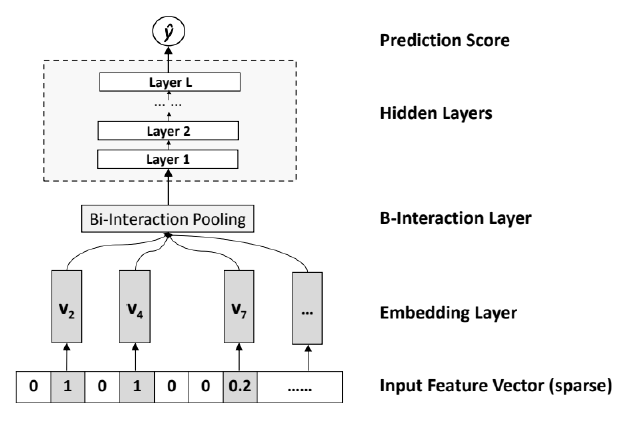
\includegraphics[width=0.7\linewidth]{figures/63.png}
\end{figure}\\
Do Embedding layer tương tự như FM nên ta sẽ tiếp tục tìm hiểu về Bi-Interaction pooling, Hidden layer, Prediction layer.

\textbf{Bi-interaction pooling:} chuyển đổi tất các embedding vectors $V_x$ thành 1 vector như sau:
$$ f_{BI}(V_x) = \sum_{i=1}^{n} \sum_{j=i+1}^{n} x_i v_i \odot x_j v_j $$
Trong đó, $\odot$ là ký hiệu của element-wise product của 2 vectors; $x_i$, $x_j$ lần lượt 
là phần tử thứ $i$ và $j$ trong feature vector $\mathbf{x}$. $\mathbf{v}_i, \mathbf{v}_j$ lần lượt là embedding của feature thứ $i$ và $j$.
\textbf{Hidden layer:} Trên Bi-interaction pooling là 1 chồng các lớp fully connected, thứ có khả năng mô hình các tương tác bậc cao giữa các đặc trưng. 
Mỗi hidden layer sẽ có một non-linear activation function như tanh, sigmoid, ReLU.
\textbf{Prediction layer:} Cuối cùng, vector đầu ra của hidden layer cuối sẽ được chuyển đổi thành prediction score:
$$f(\mathbf{x}) = \mathbf{h}^T \mathbf{z}_L$$
Trong đó, $\mathbf{h}$ là weight của prediction layer, $\mathbf{z}_L$ là output vector của hidden layer cuối.

\section{Phương pháp đề xuất}
\section{Thực nghiệm}
\subsection{Miêu tả bộ dữ liệu}
\subsection{phương pháp tổ chức dữ liệu thực nghiệm}
\subsubsection{Dịch bảng}
Trong quá trình chuyển ngữ từ Trung sang Việt, chúng em đã tận dụng thư viện "googletrans" - một công cụ Python không mất phí và không giới hạn số lần dịch. Thư viện này vận hành thông qua API Google Translate Ajax để thực hiện các tác vụ như nhận diện ngôn ngữ và dịch thuật.\\
\\
Do khối lượng dữ liệu lớn, quá trình dịch gặp phải một số thách thức về thời gian và kết nối. Để khắc phục, chúng em đã triển khai các giải pháp sau:
\begin{quote}
\begin{itemize}
    \item Lưu lại tiến trình dịch để tránh mất dữ liệu
    \item Thiết lập cơ chế tự động gửi lại yêu cầu khi mất kết nối
    \item Ứng dụng thư viện "asyncio" cho phép gửi đồng thời nhiều API, giúp tối ưu tốc độ xử lý
\end{itemize}
\end{quote}
Đây là một phần code mẫu đã sử dụng phương pháp đã nêu trên:\\
\begin{figure}[h]
    \centering
    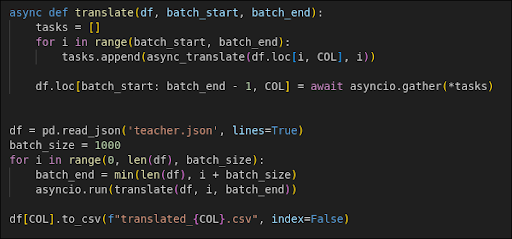
\includegraphics[width=0.75\linewidth]{figures/1.png}
\end{figure}
\newpage
Ngoài ra, chúng em nhận thấy không cần thiết phải dịch toàn bộ các trường dữ liệu lớn để huấn luyện mô hình vì một số trường dữ liệu không hỗ trợ cho việc huấn luyện mô hình. Thay vào đó, chúng em chỉ tập trung dịch 1 số trường sau đây:
\begin{quote}
-\textbf{course.json:} dịch cột “name”, “field”, “prerequisites” và “about”\\
\begin{figure}[h]
    \centering
    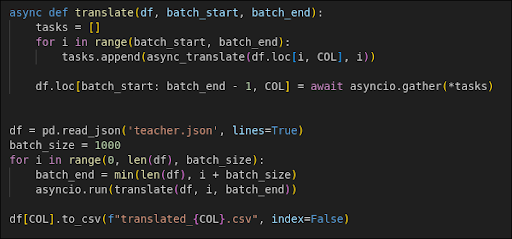
\includegraphics[width=1\linewidth]{figures/2.png}
\end{figure}\\
\\
\\
-\textbf{user.json:} dịch cột “school”\\
\begin{figure}[h]
    \centering
    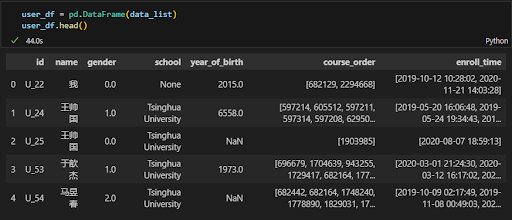
\includegraphics[width=0.8\linewidth]{figures/3.png}
\end{figure}
\newpage
-\textbf{teacher.json:} Tiến hành dịch tất cả (trừ “id” và “name”)\\
\begin{figure}[h]
    \centering
    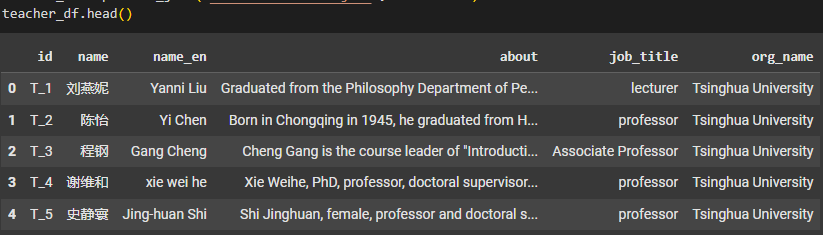
\includegraphics[width=1\linewidth]{figures/4.png}
\end{figure}\\
-\textbf{concept.json:} Dịch tất cả các cột của bảng này vì toàn bộ đều ở dạng chuỗi\\
\begin{figure}[h]
    \centering
    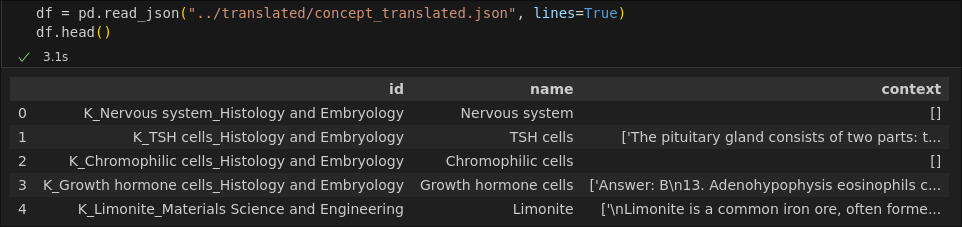
\includegraphics[width=1\linewidth]{figures/5.png}
\end{figure}\\
-\textbf{course-field.json:} Tiến hành dịch cột course\_name và field mang các thông tin dưới dạng chuỗi của bảng.\\
\begin{figure}[h]
    \centering
    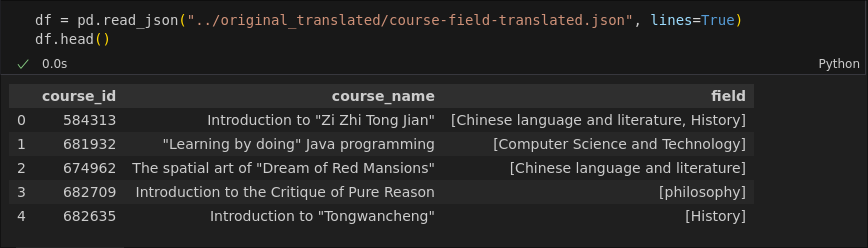
\includegraphics[width=1\linewidth]{figures/6.png}
\end{figure}
\end{quote}
\subsubsection{Khám phá dữ liệu}
\textbf{a) Bảng course.json}\\
Ta xem qua bảng course.json:
\begin{figure}[h]
    \centering
    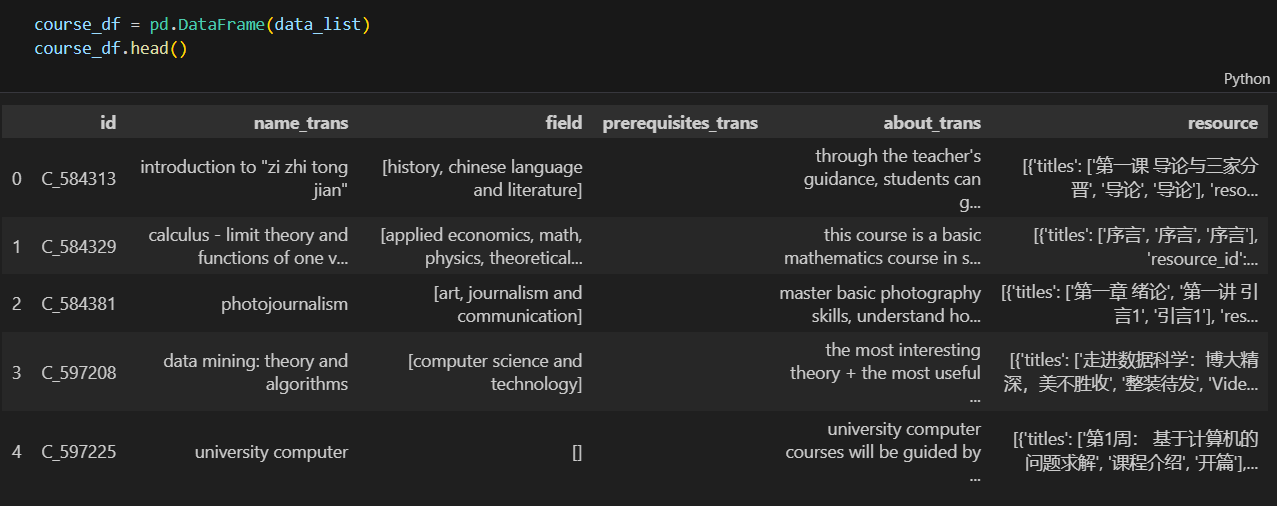
\includegraphics[width=1\linewidth]{figures/7.png}
\end{figure}\\
Ta xét độ dài của 3 cột “about”, “name\_trans” và “resource”:
\begin{figure}[h]
    \centering
    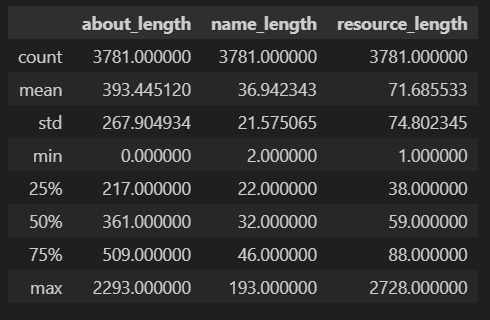
\includegraphics[width=0.485\linewidth]{figures/8.png}
\end{figure}
\newpage
Ta có thể thấy được 1 số thông tin từ dữ liệu trên:
\begin{itemize}
    \item Có những dòng dữ liệu không tồn tại cột “about”, tồn tại giá trị ngoại tệ ở cột “about” vì mean là 393 mà max lên đến 2293. Ta thể hiện trên boxplot độ dài của cột “about”:
    \begin{figure}[h]
        \centering
        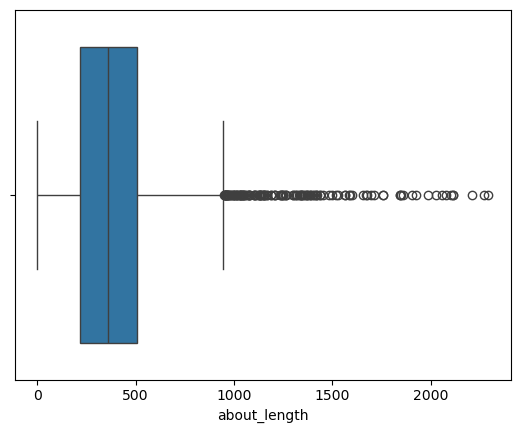
\includegraphics[width=0.75\linewidth]{figures/9.png}
    \end{figure}
    \item Có thể thấy thật sự nhiều giá trị ngoại tệ cần được xử lí.
    \item Có những dòng dữ liệu không có resource\_length, mean cũng rất ngắn (71) chứng tỏ ít thông tin về khoá học.
\end{itemize}
Ta phân tích sâu cột “resource”:
\begin{figure}[h]
    \centering
    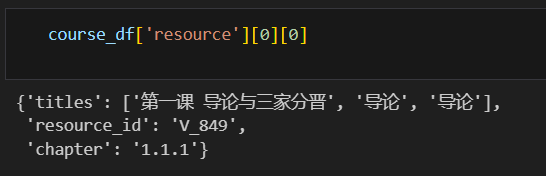
\includegraphics[width=0.75\linewidth]{figures/10.png}
\end{figure}\\
Mỗi resource trong bảng 2 là 1 tập hợp các video hay một tập các exercise. Mỗi resource sẽ có thêm 1 resource\_id là id của resource, chapter là chương chứa resource trong khóa học, titles gồm các tiêu đề như tiêu đề chương, video chương.\\
\\
Thông tin của resource có thể tìm thấy trong file course.json. Một resource có 2 loại: Video và Exercise. Nếu loại tài nguyên là video, nó được xác định bằng ID video bắt đầu bằng ký tự V\_. Nhiều video\_id khác nhau tương ứng với một ccid, và ccid xác định duy nhất một video. Các video\_id này tương ứng với việc hiển thị cùng một video ccid tại các thời gian bắt đầu khác nhau. Mối liên hệ giữa video\_id và ccid được lưu trong relations/video\_id-ccid.txt. Phụ đề video có thể được tìm thấy trong tệp entities/video.json thông qua ccid.\\
\\
Ta sẽ kiểm tra xem có bao nhiêu ID video không hợp lệ để phục vụ cho quá trình xử lý dữ liệu sau này:
\begin{figure}[h]
    \centering
    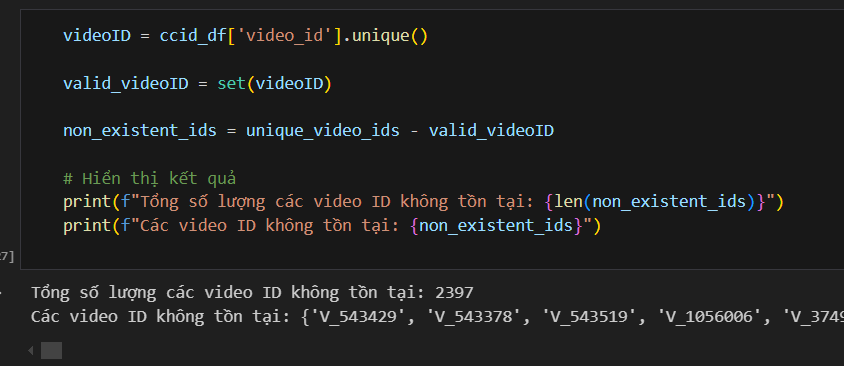
\includegraphics[width=0.75\linewidth]{figures/11.png}
\end{figure}\\
Có 2397 video ID không tồn tại, ta sẽ lọc đi hỗ trợ cho hiển thi thông tin trong tương lai.\\
\\
Ta bắt đầu tiến hành đếm số khoá học trong cột “name\_trans”, chia bởi lĩnh vực (cột “field”):\\
\begin{figure}[h]
    \centering
    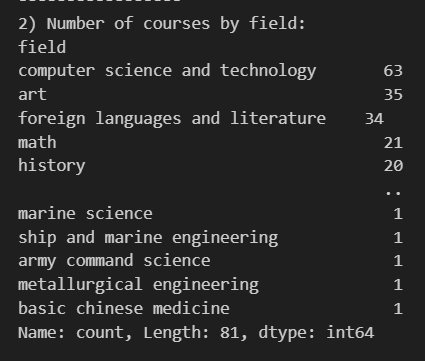
\includegraphics[width=0.35\linewidth]{figures/12.png}
\end{figure}
\newpage
\begin{figure}
    \centering
    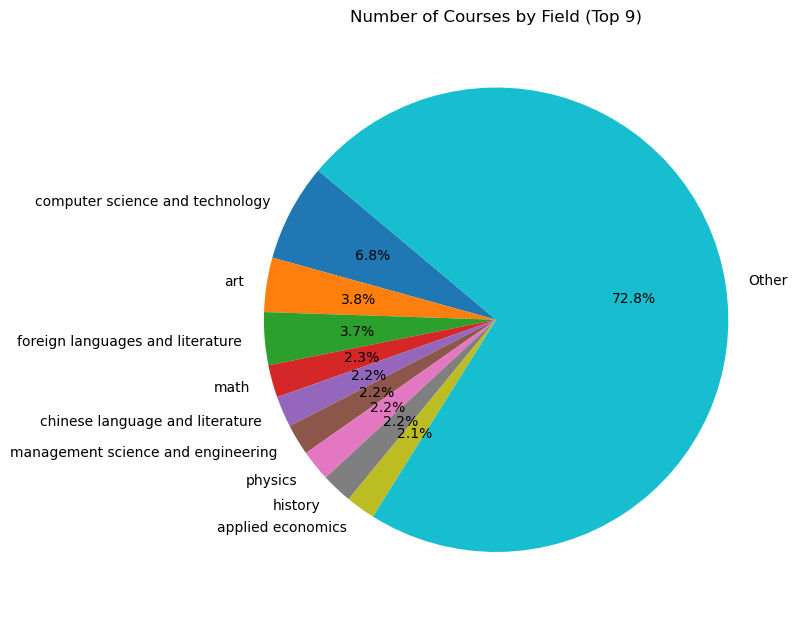
\includegraphics[width=0.7\linewidth]{figures/13.png}
\end{figure}
Ta thấy có tổng 3781 khoá học và 81 lĩnh vực, với “computer science and technology” đứng đầu với 63 khoá học, chiếm 6.8\% trên tổng khoá học. Ta cũng kiểm tra với mỗi khoá học được xếp bao nhiêu lĩnh vực (cột “field”):
\begin{figure}[h]
    \centering
    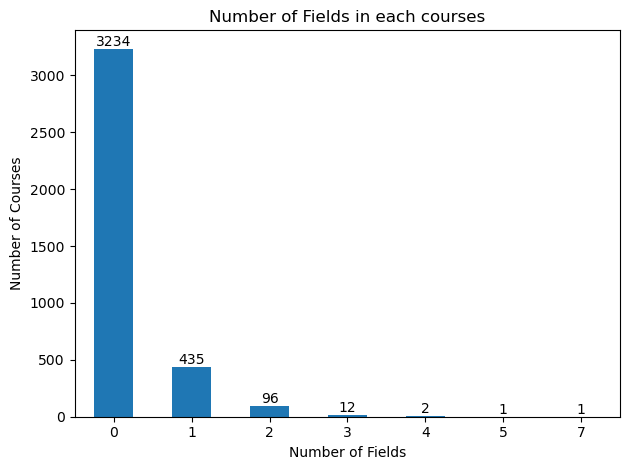
\includegraphics[width=0.9\linewidth]{figures/14.png}
\end{figure}\\
\newpage
Ta có thể thấy có rất nhiều khoá học không thuộc lĩnh vực nào, có rất nhiều khóa học không có field nào, có thể cột “field” sẽ không đóng góp nhiều trong xây dựng thuật toán hoặc cần xử lí.\\
\textbf{b) Bảng user.json}\\
Đầu tiên, ta đọc dữ liệu và quan sát dữ liệu thông qua dạng bảng (DataFrame):
\begin{figure}[h]
    \centering
    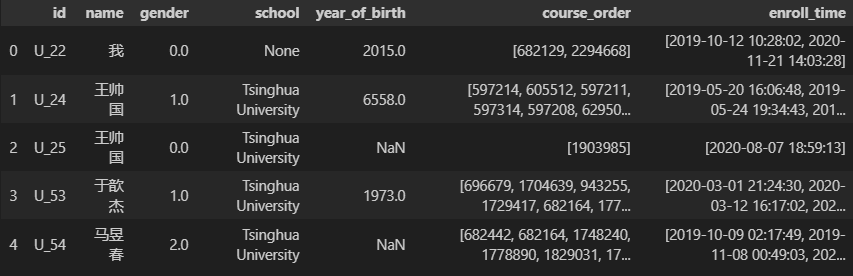
\includegraphics[width=1\linewidth]{figures/15.png}
\end{figure}
\newpage
Ta tiến hành thống kê đặc điểm từng cột có trong bảng:
\begin{figure}[h]
    \centering
    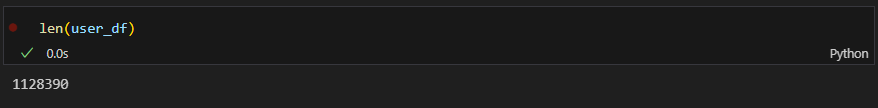
\includegraphics[width=1\linewidth]{figures/16.png}
    \caption{Số lượng users}
\end{figure}
\begin{figure}[h]
    \centering
    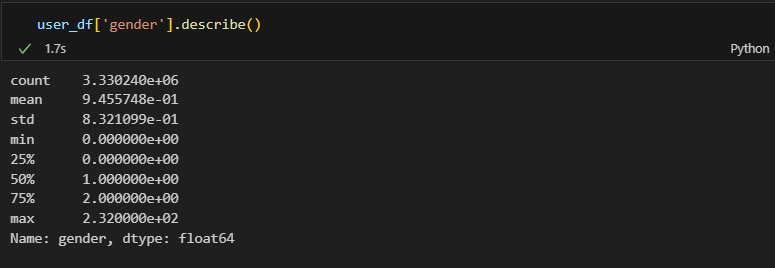
\includegraphics[width=1\linewidth]{figures/17.png}
    \caption{Cột “gender”}
\end{figure}
\begin{figure}[h]
    \centering
    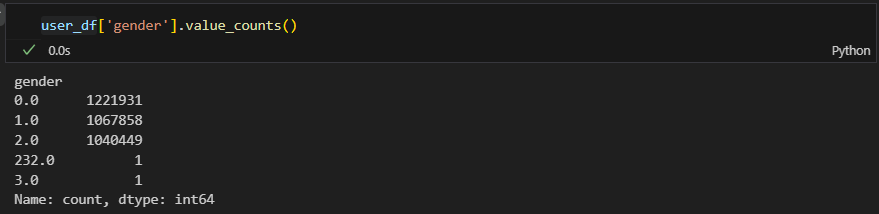
\includegraphics[width=1\linewidth]{figures/18.png}
    \caption{Phân bố các các giá trị trong cột “gender”:}
\end{figure}
\newpage
\begin{figure}
    \centering
    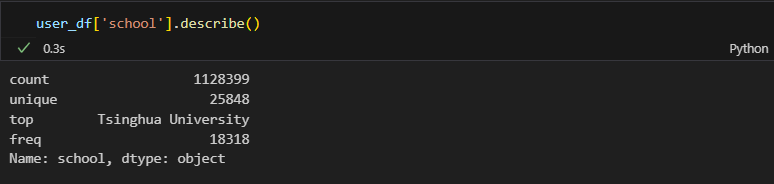
\includegraphics[width=1\linewidth]{figures/19.png}
    \caption{Thông tin cột “school”}
\end{figure}
\begin{figure}[h]
    \centering
    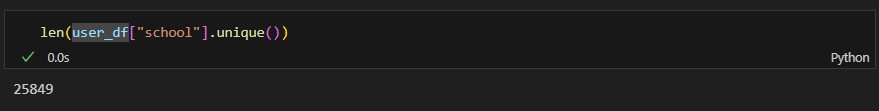
\includegraphics[width=1\linewidth]{figures/20.png}
    \caption{Số lượng trường học trong bảng}
\end{figure}
\begin{figure}[h]
    \centering
    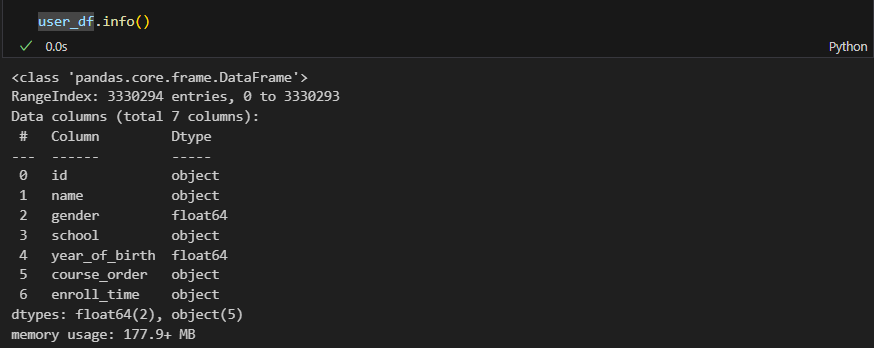
\includegraphics[width=1\linewidth]{figures/21.png}
    \caption{Kiểm tra thông tin tổng quan sau cùng}
\end{figure}
\newpage
\begin{figure}
    \centering
    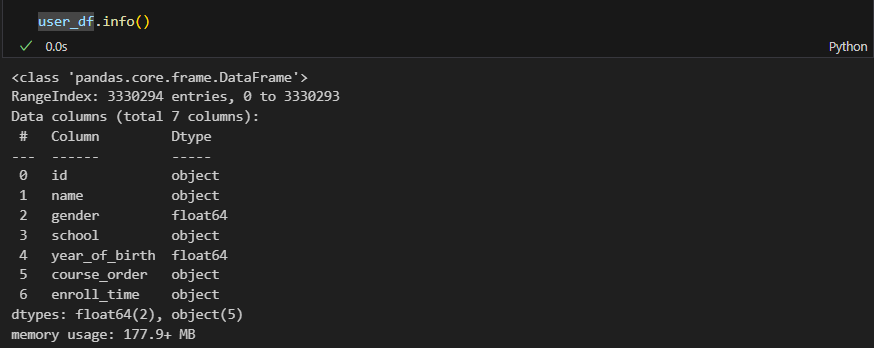
\includegraphics[width=1\linewidth]{figures/22.png}
    \caption{Số lượng sample (users) có trong bảng và số lượng users thuộc về mỗi trường học}
\end{figure}
\begin{figure}[h]
    \centering
    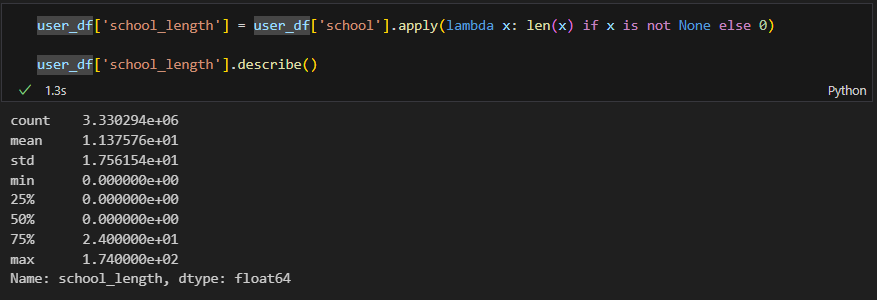
\includegraphics[width=1\linewidth]{figures/23.png}
    \caption{Tạo một cột “school\_length” để phân tích độ dài mỗi sample của cột}
\end{figure}
\newpage
\begin{figure}
    \centering
    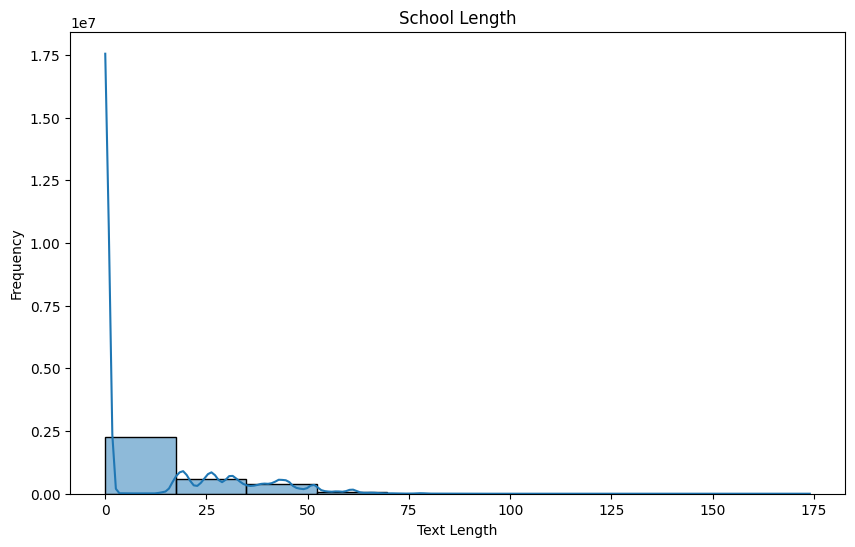
\includegraphics[width=0.68\linewidth]{figures/24.png}
    \caption{Trực quan hóa độ dài của sample cột “school”}
\end{figure}
\begin{figure}[h]
    \centering
    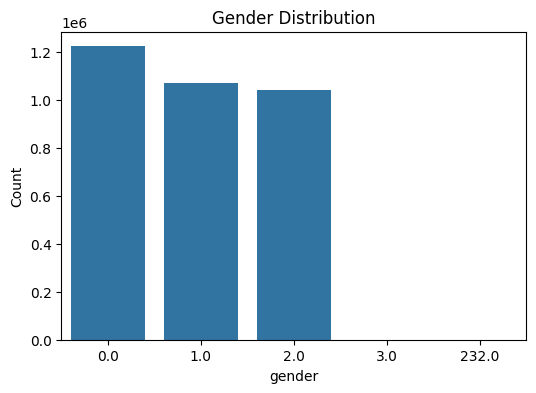
\includegraphics[width=0.68\linewidth]{figures/25.png}
    \caption{Trực quan hóa phân bố các giá trị của cột “gender”}
\end{figure}
\newpage
\textbf{c) Bảng teacher.json}\\
Sau đây là các thống số cơ bản của bảng
\begin{figure}[h]
    \centering
    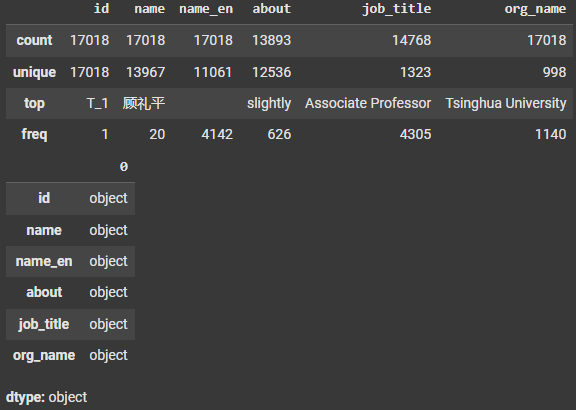
\includegraphics[width=0.6\linewidth]{figures/27.png}
\end{figure}\\
Tham khảo phân phối của top 10 tên việc xuất hiện nhiều nhất trong bảng
\begin{figure}[h]
    \centering
    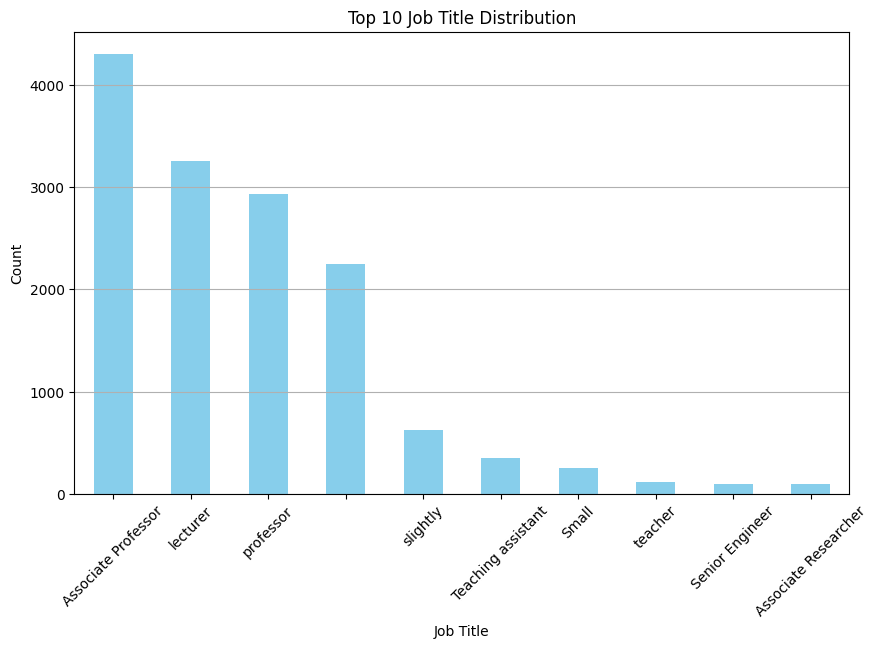
\includegraphics[width=0.75\linewidth]{figures/28.png}
\end{figure}\\
Tham khảo phân phối của top 10 tổ chức xuất hiện nhiều nhất trong bảng
\newpage
\begin{figure}
    \centering
    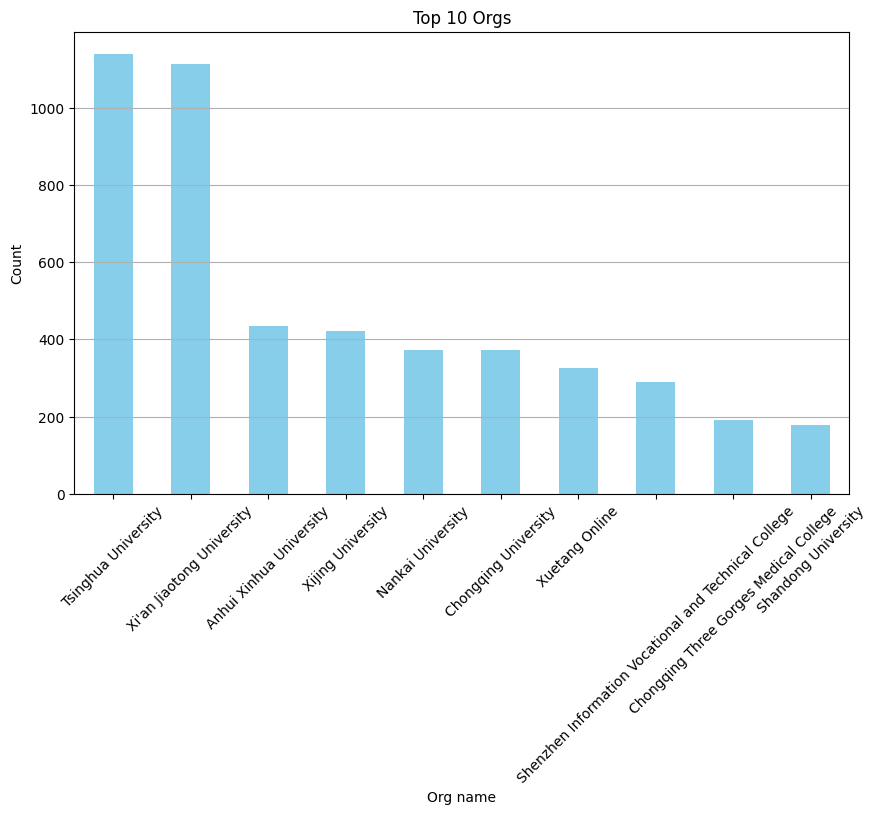
\includegraphics[width=0.75\linewidth]{figures/29.png}
\end{figure}
Ta thực hiện phân tích mối quan hệ giữa ba chức vụ (job titles) có số lượng giáo viên nhiều nhất và mười tổ chức (organizations) có số lượng giáo viên cao nhất
\begin{figure}[h]
    \centering
    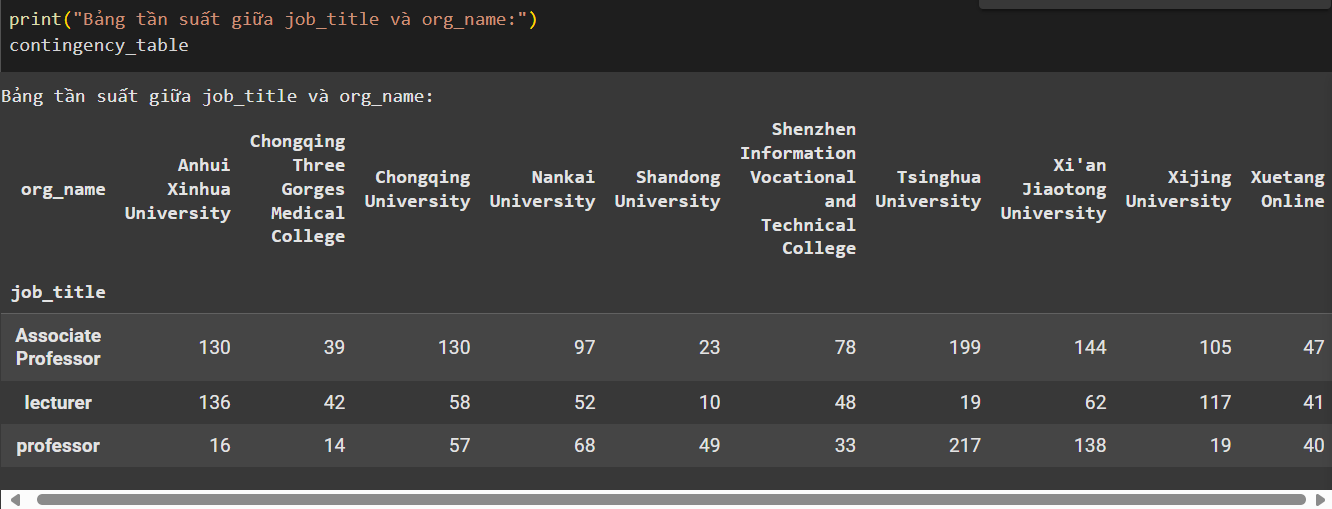
\includegraphics[width=0.95\linewidth]{figures/30.png}
\end{figure}
\newpage
\begin{figure}
    \centering
    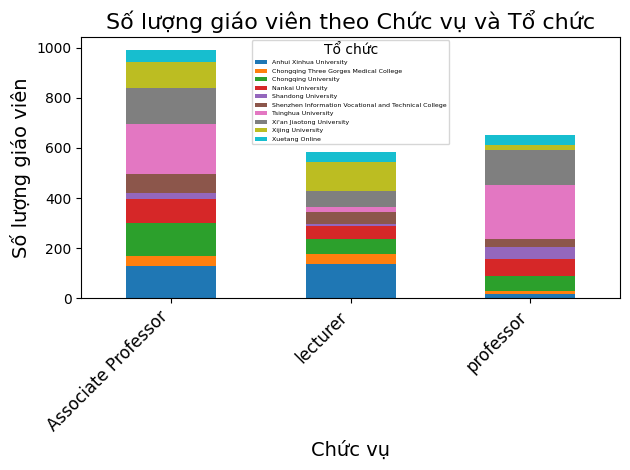
\includegraphics[width=0.65\linewidth]{figures/31.png}
\end{figure}
Sau khi lọc bỏ các liên kết có khóa học hoặc teacher không tồn tại dựa vào file course-teacher.txt, số hàng còn lại là 35593. Các thông tin được trực quan hóa như sau
\begin{figure}[h]
    \centering
    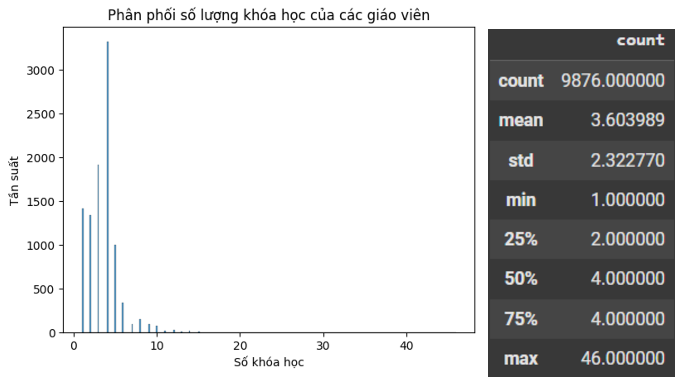
\includegraphics[width=0.8\linewidth]{figures/32.png}
    \caption{Histogram thể hiện số lượng khóa học của mỗi teacher và bảng thống kê mô tả tương ứng}
\end{figure}
\newpage
\begin{figure}
    \centering
    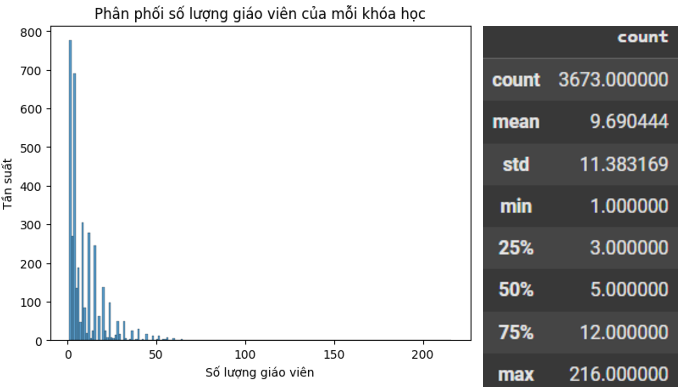
\includegraphics[width=0.8\linewidth]{figures/33.png}
    \caption{Histogram thể hiện số lượng teacher của mỗi khóa học và bảng thống kê mô tả tương ứng}
\end{figure}
\textbf{d) Bảng school.json}\\
Ta đếm dữ liệu ở từng cột, đếm các giá trị đặc biệt, giá trị xuất hiện nhiều nhất với tần số của nó:
\begin{figure}[h]
    \centering
    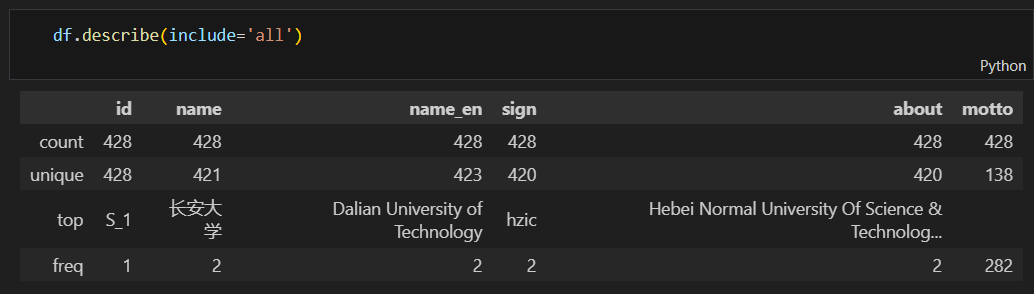
\includegraphics[width=0.75\linewidth]{figures/34.png}
\end{figure}\\
Kiểm tra kiểu dữ liệu của từng cột: 
\newpage
\begin{figure}
    \centering
    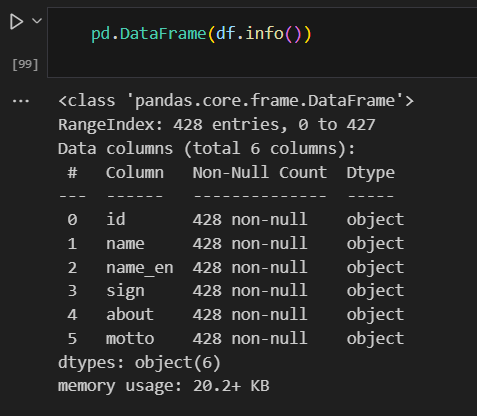
\includegraphics[width=0.6\linewidth]{figures/35.png}
\end{figure}
Ta tạo 2 cột mới là “about\_length” và “motto\_length” để lần lượt thể hiện độ dài của giá trị dữ liệu ở 2 cột “about” và “motto”:
\begin{figure}[h]
    \centering
    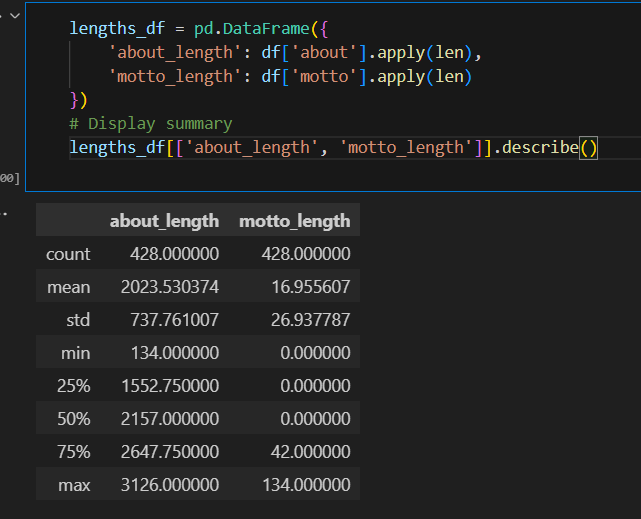
\includegraphics[width=0.65\linewidth]{figures/36.png}
\end{figure}
\newpage
Có 2 cột ta cần là “about\_length” và “motto\_length” để ta tìm phân bố độ dài của giá trị lên đồ thị:
\begin{figure}[h]
    \centering
    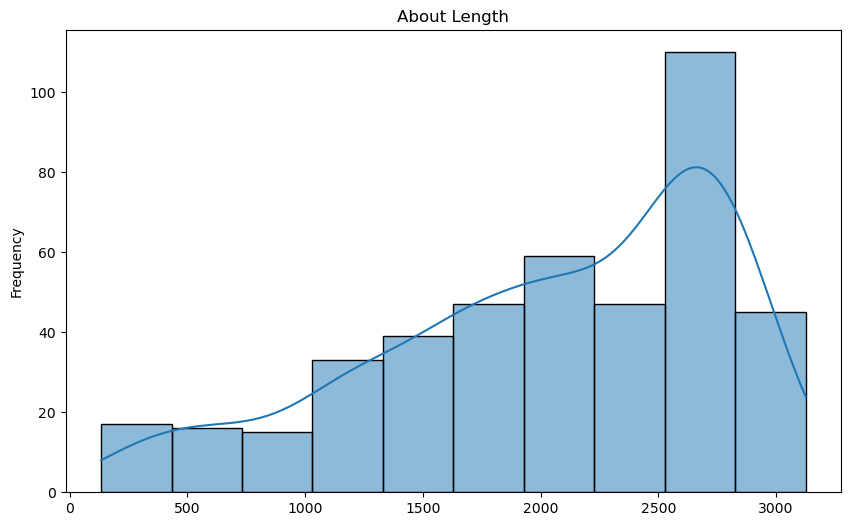
\includegraphics[width=0.7\linewidth]{figures/37.png}
\end{figure}\\
Dựa vào biểu đồ ta có thể nhận xét rằng mô tả của các trường đều rất chi tiết, số lượng trường với số lượng từ phần mô tả > 2000  chiếm phần lớn. Tuy nhiên thông tin này có vẻ không hữu ích với hệ thống khuyến nghị.
\begin{figure}[h]
    \centering
    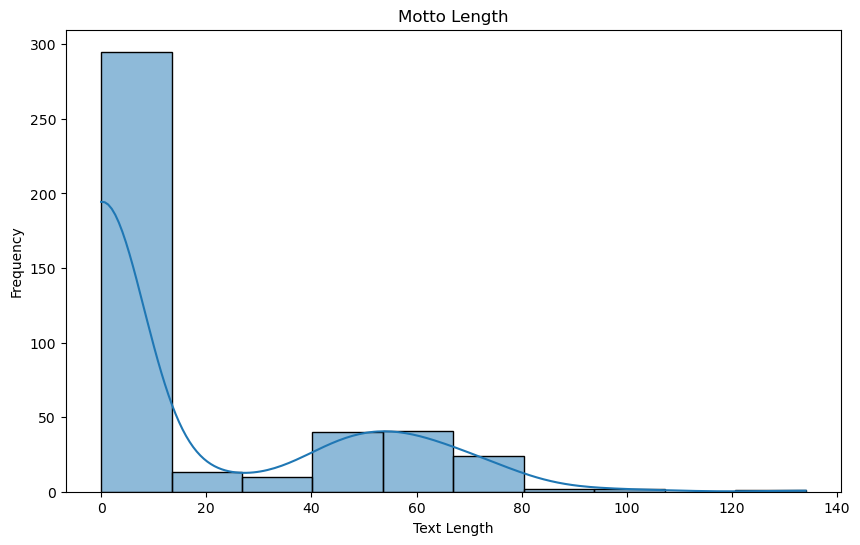
\includegraphics[width=0.7\linewidth]{figures/38.png}
\end{figure}\\
Hầu hết các trường đại học đều có một khẩu hiệu ngắn gọn dưới 20 từ vì chủ yếu khẩu hiệu sẽ đơn giản nhất có thể để truyền đạt tầm nhìn và mục tiêu của trường một cách trực tiếp ngắn gọn, đọng lại trong trí nhớ người xem. Một phần nhỏ hơn các trường có khẩu hiệu tương đối dài với 40 đến 88 chữ. 
\newpage
\textbf{e) Bảng course-field.json}
\begin{figure}[h]
    \centering
    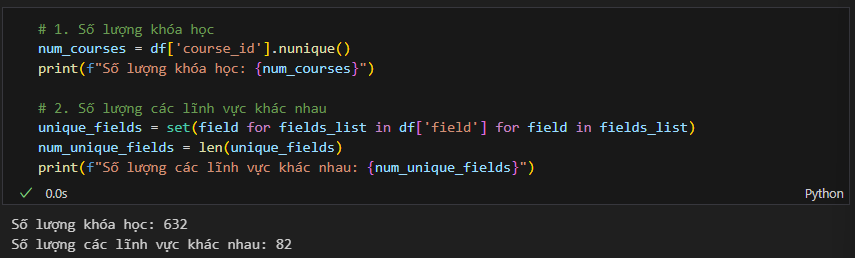
\includegraphics[width=1\linewidth]{figures/39.png}
    \caption{Tổng số lượng khóa học và tổng số lượng các lĩnh vực khác nhau}
\end{figure}
\begin{figure}[h]
    \centering
    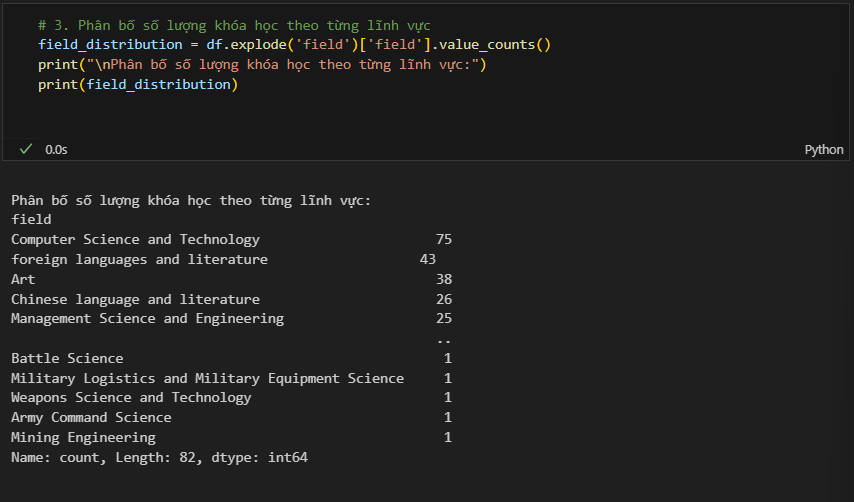
\includegraphics[width=1\linewidth]{figures/40.png}
    \caption{Phân bố số lượng khóa học theo từng lĩnh vực}
\end{figure}
\newpage
\begin{figure}
    \centering
    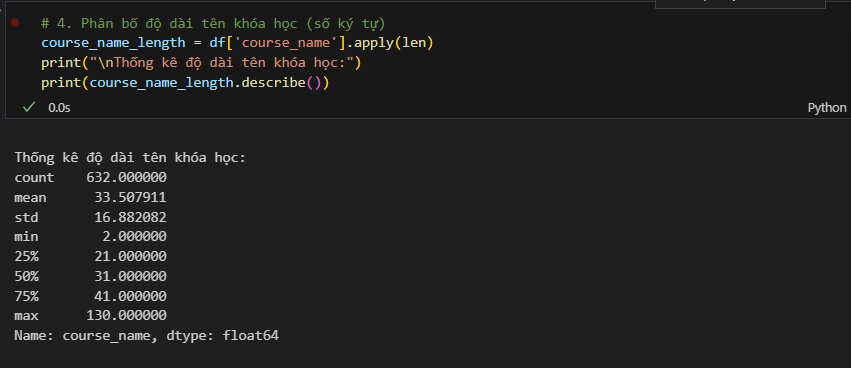
\includegraphics[width=0.85\linewidth]{figures/41.png}
    \caption{Phân bố độ dài tên khóa học}
\end{figure}
\begin{figure}[h]
    \centering
    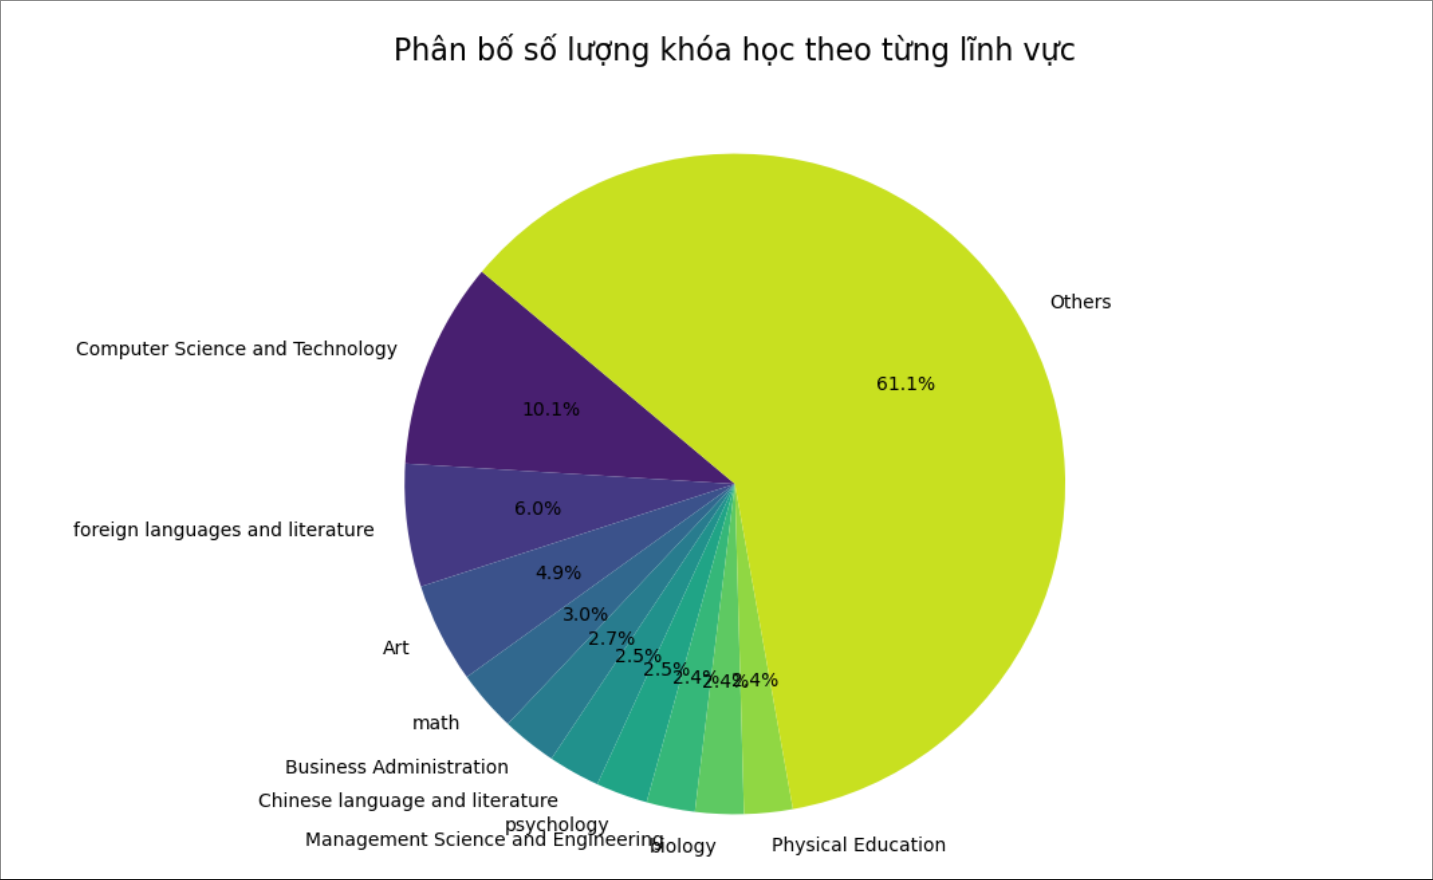
\includegraphics[width=0.9\linewidth]{figures/42.png}
    \caption{Biểu đồ thanh thể hiện sự phân bố số lượng khóa học theo từng lĩnh vực}
\end{figure}
\newpage
\begin{figure}
    \centering
    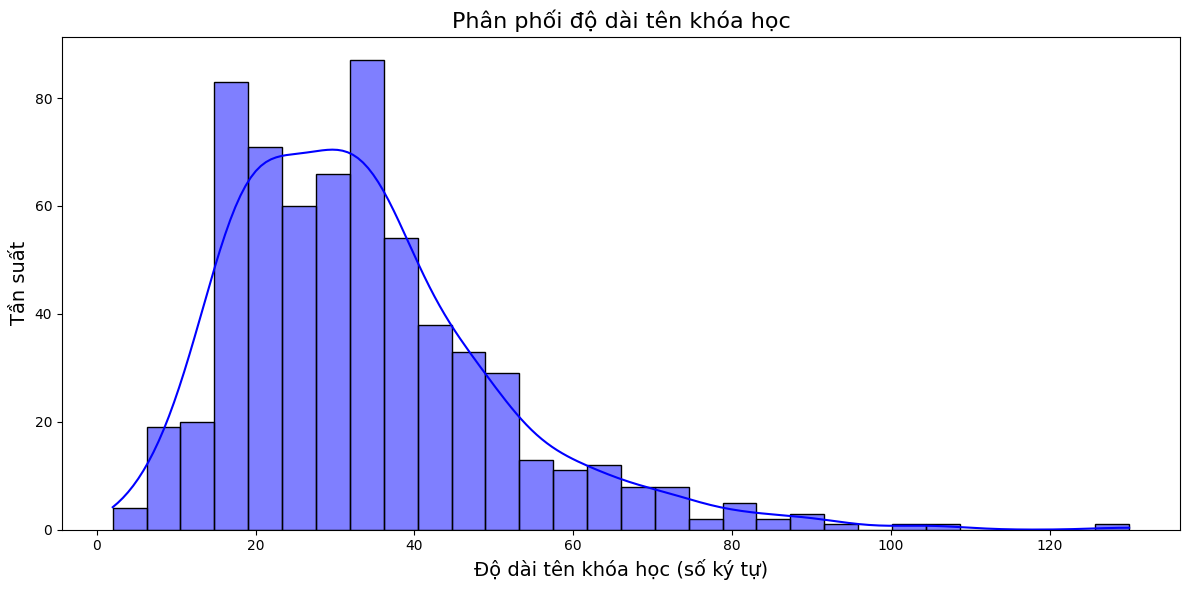
\includegraphics[width=0.75\linewidth]{figures/44.png}
    \caption{Biểu đồ phân phối cho độ dài tên khóa học}
\end{figure}
\subsubsection{Làm sạch dữ liệu}
\textbf{a) Bảng course.json}\\
Ta kiểm tra dữ liệu thiếu, dữ liệu không nhất quán, dữ liệu trùng lặp và dữ liệu trống:
\\
Đầu tiên ta thấy được có 647 giá trị ở cột “name\_trans” bị trùng lặp cho dù id không bị trùng, chứng tỏ có sự lỗi nhất định trong bộ dữ liệu, cũng như nãy đã thống kê ta thấy được có rất nhiều giá trị trống ở cột “field\_trans”.\\
\\
Ta kiểm tra kĩ hơn về các dòng có giá trị trong cột “name” bị trùng lặp:
\begin{figure}[h]
    \centering
    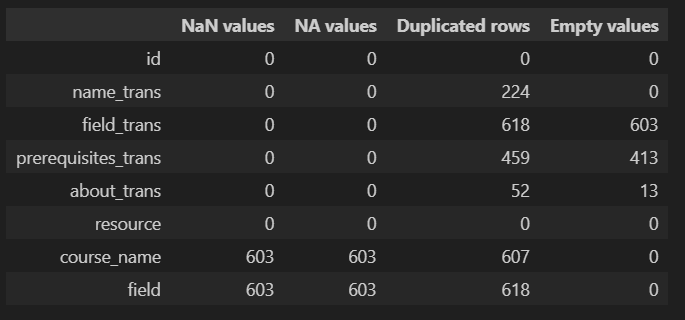
\includegraphics[width=1\linewidth]{figures/26.png}
\end{figure}
\newpage
\begin{figure}
    \centering
    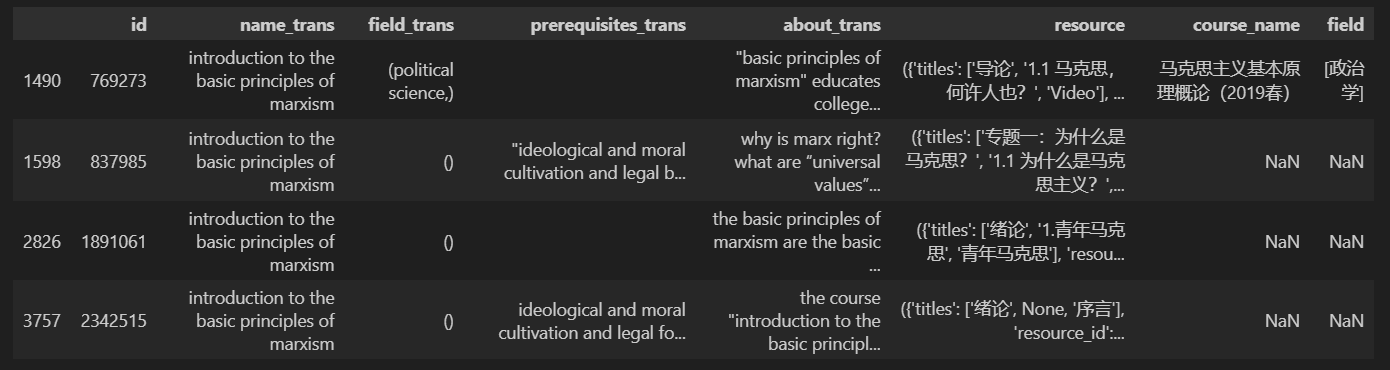
\includegraphics[width=1\linewidth]{figures/45.png}
\end{figure}
Ta thấy được đa số dữ liệu trong này cột “field” đa số bị trống và trùng lặp, cũng như các cột khác không có ý nghĩa hoặc trùng với các cột khác, thực hiện chi square test, ta có được kết quả với P-value rất thấp, chứng tỏ các giá trị phụ thuộc với nhau chứ không hề có giá trị mới. Chứng tỏ ta có thể xoá được các dòng dữ liệu này, cũng như các khoá học không tồn tại trong “course-field.json”.\\
\textbf{b) Bảng user.json}\\
Ta thấy cột “year\_of\_birth” bị thiếu dữ liệu hơn 97\% trong khi các cột còn lại tỉ lệ \% thiếu là rất thấp. Ta tiến hành loại bỏ cột này, sau đó ta sẽ tiến hành xử lý dữ liệu nhiễu trên cột gender với 2 giá trị nhiễu là 232 và 3\\
\textbf{c) Bảng concept.json}\\
Ta thấy cột “id” bị thiếu 207 giá trị, ta tiến hành bỏ các hàng này.\\
\begin{figure}[h]
    \centering
    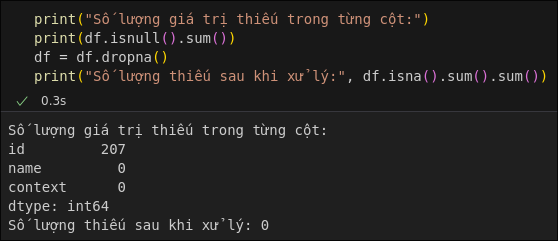
\includegraphics[width=1\linewidth]{figures/46.png}
\end{figure}
\newpage
Ta kiểm tra kĩ hơn về các bản ghi có giá trị trùng lặp và xử lý chúng:\\
\begin{figure}[h]
    \centering
    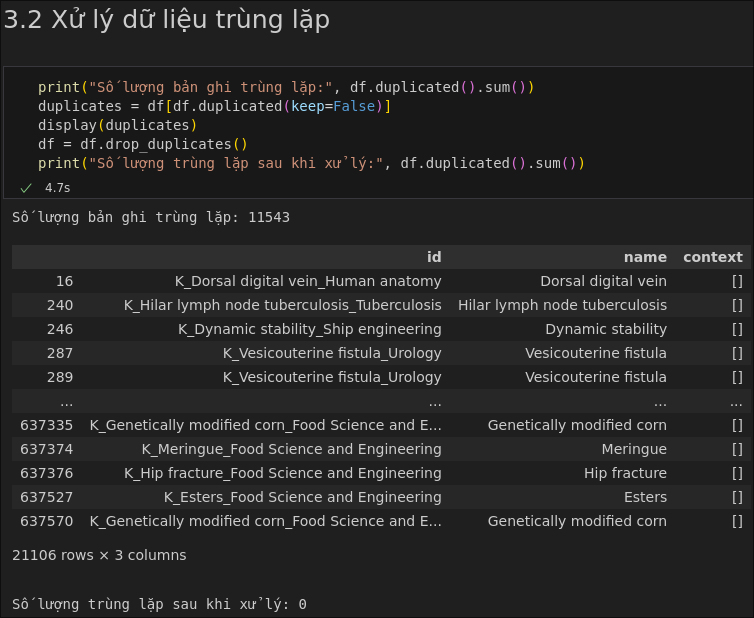
\includegraphics[width=1\linewidth]{figures/47.png}
\end{figure}\\
\textbf{d) Bảng course-field.json}\\
Sử dụng isnull().sum() để tính số lượng giá trị thiếu trong từng cột. Sau đó loại bỏ hàng chứa giá trị thiếu bằng cách sử dụng dropna()
\newpage
\begin{figure}
    \centering
    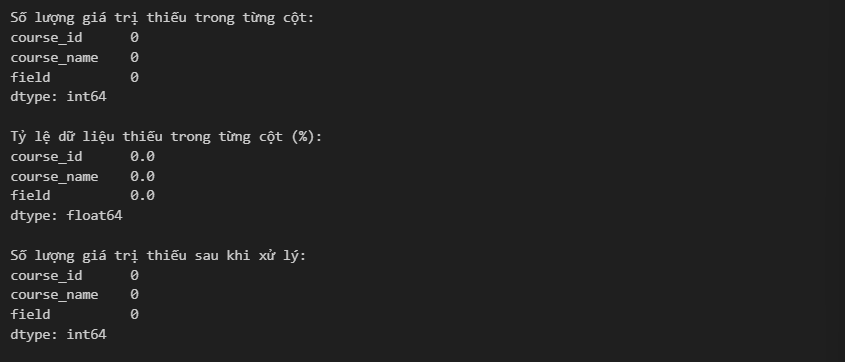
\includegraphics[width=1\linewidth]{figures/48.png}
\end{figure}
Dữ liệu văn bản thường chứa nhiều thông tin nhiễu chẳng hạn như các ký tự không mong muốn: Các ký tự đặc biệt, dấu câu, hoặc ký tự không phải chữ cái có thể làm giảm chất lượng phân tích. Ở đây chúng ta sẽ tiến hành loại bỏ các ký tự không cần thiết, các khoảng trắng dư thừa và thường hóa các ký tự viết hoa\\
\\
Để kiếm tra dữ liệu trùng lặp, chúng ta sử dụng phương thức duplicated() trong pandas. Đầu tiên xác định các bản ghi trùng lặp, sau đó đếm số lượng và hiển thị các bảng ghi trùng lặp đó. Sau đó tiến hành xóa bản ghi trùng lặp bằng cách sử dụng drop\_duplicates()
\newpage
\begin{figure}
    \centering
    \includegraphics[width=1\linewidth]{figures/49.png}
\end{figure}
\textbf{e) Bảng school.json}\\
Ta xoá cột “name” đi vì trùng với ý nghĩa với cột “name\_en” (tên nhưng trong Tiếng Anh)\\
\\
Ta thống nhất cột “sign” (kí hiệu đại diện cho trường) đều là tất cả in hoa:
\newpage
\begin{figure}
    \centering
    \includegraphics[width=0.7\linewidth]{figures/50.png}
\end{figure}
Vì ở đây tên trường (“name\_en”) cũng như kí hiệu (“sign”) là chìa khoá chính, hay nói cách khác là giá trị duy nhất nên không thể có dòng trùng với nhau, ta tiến hành xoá các dòng trùng giá trị:
\begin{figure}[h]
    \centering
    \includegraphics[width=0.7\linewidth]{figures/51.png}
\end{figure}\\
\textbf{g) Bảng teacher.json}\\
Ở đây có cột name\_en bị thiếu nên điền vào cột đó bằng cách lấy phiên âm của cột name là được. Để làm việc này có thể sử dụng thư viện pypinyin để lấy phát âm dùng cho tên tiếng anh.
\newpage
\begin{figure}
    \centering
    \includegraphics[width=0.8\linewidth]{figures/52.png}
\end{figure}
\subsubsection{Chuyển đổi dữ liệu}
\textbf{Feature Engineering:}
Nhóm sẽ chọn các bảng và thuộc tính có thể sử dụng để tạo ra feature các mô hình khuyến nghị dựa trên bộ dữ liệu đã xử lý và làm sạch trước đó:\\
\\
Các bảng được chọn và thuộc tính sử dụng:
\begin{figure}[h]
    \centering
    \includegraphics[width=0.6\linewidth]{figures/53.png}
\end{figure}
\newpage
\begin{itemize}
    \item Với ‘user.json’: ‘course\_order’ gồm các khóa học mà user đã đăng ký với khóa học sau cùng là khóa học gần đây nhất, dùng để tạo liên kết giữa ‘user.json’ và ‘course.json’.
    \item Với ‘course.json’: Đây là table quan trọng chứa thông tin về các khóa học như ‘name’, ‘about’ và ‘field’.
    \item Với ‘teacher.json’, ‘school.json’: dùng để tạo relation với ‘course.json’ chứa thông tin về trường tổ chức khóa học và giáo viên giảng dạy.
    \item Với ‘course-field.json’: chứa các field của mỗi khóa học, dùng để kiểm tra với trường ‘field’ trong ‘course.json’.
    \item Với ‘concept.json’: id theo quy ước ‘K\_{concept name}{field}’, tạo thêm feature concept-name\_field với mỗi khoá học.
\end{itemize}
Tạo knowledge graph:
\begin{figure}[h]
    \centering
    \includegraphics[width=0.3\linewidth]{figures/54.png}
\end{figure}\\
Tạo interaction giữa người dùng với khóa học: sử dụng 5-core filtering, lọc người dùng với ít hơn 5 khóa học và những khóa học có số lượng đăng ký dưới 5.\\
\\
Kết quả: Vì data đã được xử lý trước đó nên ta thấy không có thay đổi đáng kể
\begin{center}
\begin{tabular}{|| m{15em}  m{15em}||} 
 \hline
 Trước khi filter & Sau khi filter\\ [0.5ex] 
 \hline\hline
 1.183.774 interactions & 1.182.745 interactions \\ [1ex]
 \hline
\end{tabular}
\end{center}
\newpage
Tạo relation giữa các entities: course-relation-attribute. Sau đó ta tiến hành lọc theo tiêu chí, số lần course xuất hiện tối thiểu là 5 và số lần xuất hiện tối thiểu của một relation là 25. \\
\\
Kết quả: 
\begin{center}
\begin{tabular}{|| m{15em}  m{15em}||} 
 \hline
 Trước khi filter & Sau khi filter\\ [0.5ex] 
 \hline\hline
 376.093 interactions & 71.787 interactions \\ [1ex]
 \hline
\end{tabular}
\end{center}
\subsubsection{Chia tập dữ liệu}
\begin{itemize}
    \item Dữ liệu cuối cùng được chia theo chiến lược leave-one-out: Với mỗi user, nhóm giữ khoá học cuối cùng làm test, các khoá học còn lại làm train. 
    \item Dữ liệu cuối cùng để thực nghiệm có 4 loại dữ liệu chính: dữ liệu thô (chưa xử lí), 10\% dữ liệu thô, dữ liệu đã xử lí (chiến lược leave-one-out) và 10\% dữ liệu đã xử lí.
\end{itemize}

\subsection{Độ đo đánh giá}
\subsection{Kịch bản thực nghiệm}
\subsection{Đánh giá kết quả thực nghiệm}

\section{Kết luận và hướng phát triển}

\newpage



% ----------------------------------------------------------------------------------------
\end{document}
